\documentclass{article}
\usepackage{amsmath}
\usepackage{amssymb}
\usepackage{graphicx}
\usepackage{hyperref}
\usepackage[version=4]{mhchem}

\title{Example 7}
\date{}

\begin{document}
\maketitle

(AMC) In triangle \(A B C\) lines \(C E\) and \(A D\) are drawn so that \(\frac{C D}{D B}=\frac{3}{1}\) and \(\frac{A E}{E B}=\frac{3}{2}\). Let \(r=\frac{C P}{P E}\), where \(P\) is the intersection point of \(C E\) and \(A D\). Then \(r\) equals:\\
(A) 3\\
(B) \(\frac{3}{2}\)\\
(C) 4\\
(D) 5\\
(E) \(\frac{5}{2}\)\\
\centering
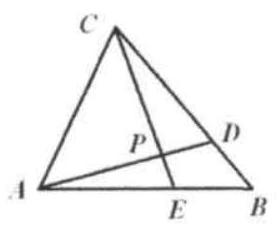
\includegraphics[width=\textwidth]{images/problem_image_1.jpg}

Solution: (D).


Draw \(D R / / A B . \frac{C R}{R E}=\frac{C D}{D B}=\frac{3}{1}, \frac{R D}{E B}=\frac{C D}{D B}=\frac{3}{4}\);\\
\(\therefore C R=3 R E=3 R P+3 P E\) and \(R D=\frac{3}{4} E B\),\\
\(\therefore C P=C R+R P=4 R P+3 P E\)\\
\centering
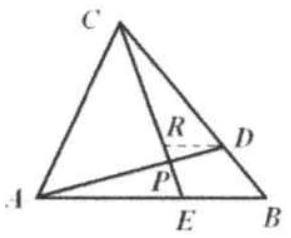
\includegraphics[width=\textwidth]{images/reasoning_image_1.jpg}

Since \(\triangle R D P \sim \triangle E A P, \frac{R P}{P E}=\frac{R D}{A E}, \quad \therefore R D=\frac{R P \times A E}{P E}\).\\
\(\therefore R D=\frac{R P}{P E} \cdot \frac{3}{2} E B . \therefore \frac{3}{4} E B=\frac{3}{2} E B \cdot \frac{R P}{P E}, \quad \therefore R P=\frac{1}{2} P E\), \(C P=4 \cdot \frac{1}{2} P E+3 P E=5 P E ; \therefore \frac{C P}{P E}=5\).


\end{document}
